\documentclass[main.tex]{subfiles}
\setlength{\columnsep}{3cm}
\begin{document}

\addtolength{\tabcolsep}{-2pt}

\section{Exploiting Parallelism on a Single Core}
In the last chapter, we talked about how to use the Java thread library, how threads can communicate and solve different problems related to organizing concurrency.\\
Until now, our parallelization approach was the following: We have a sequential program and decide as programmers that some parts can be executed concurrently. So we create a new Java Thread object and let it execute this code part concurrently. What we assume there is that we have multiple \textit{cores} that can execute multiple threads in parallel. This kind of parallelism is exploited by the programmer itself.\\
However, some clever tricks can also be applied to get parallelism on a \textit{single} core out of a program. These are generally abstracted away from the programmer and require special hardware support.

\subsection{Instruction-Level Parallelism (ILP)}
ILP refers to parallelism that can be obtained by executing independent instructions in parallel. Consider the following pseudo-assembly:
\begin{minted}[]{java}
1: ADD R1, a, b // R1 <- a + b
2: ADD R2, c, d // R2 <- c + d
3: ADD R3, R1, R2 // R3 <- R1 + R2
\end{minted}
The first two instructions are completely independent and can be executed concurrently. The third however has to wait for the first two to complete. We can exploit \textit{ILP} for the first two instructions. Generally, we say that two instructions are independent if the result of one is not the operand (or input) of the other.

\subsubsection{ILP vs Multi-Threading}

We clearly differentiate ILP from concurrency (or multi-threading): ILP concerns the execution of a \textit{single} thread, while concurrency intrinsically concerns multiple threads. Basically, we can first start multiple threads (multi-threading to exploit multiple cores on the machine) to each execute a sequential part of the program. Then, within each thread (that can itself be viewed as a sequence of instructions), we seek independent instructions that \textit{could} be executed in parallel. Now of course it is inefficient to start another thread to execute a single instruction concurrently (because of thread creation and context switch overhead). Also, assume that we already have enough threads to keep all cores busy.\\
It would be nice to execute this independent instruction in parallel \textit{within} the core the thread is alredy scheduled on. This kind of parallelism is what ILP refers to. To exploit ILP, we need additional hardware of course; if the core the thread runs on does not provide the hardware to execute multiple instructions in parallel, no software tool will be able to make it happen.\\
In the following, we will explore different approaches towards implementing ILP.

\subsection{Pipelining}
Pipelining is a very general concept; it is about partitioning a process (do not think of an OS process here) into different stages, usually each with its clear function.

\subsubsection{A Simple Example: Latency and Throughput}
Let us analyze the process of doing laundry. We can divide this into the following stages:
\begin{itemize}
  \item Washing (15 minutes)
  \item Drying (10 minutes)
  \item Folding the dry clothes (5 minutes)
  \item Put clothes back into closet (5 minutes)
\end{itemize}
Now imagine we have multiple loads of laundry we need to process. We can wait for one load to complete with all stages and then start with the next. But it would be more efficient to start with the second load as soon as the first is done with washing (the first stage) and so on. We receive the following execution:\\[3mm]
\begin{tabular}{l | *{19}{c}}
    Time (m) & 0 & 5 & 10 & 15 & 20 & 25 & 30 & 35 & 40 & 45 & 50 & 55 & 60 & 65 & 70 & 75 & 80 & 85 & 90 \\
    \hline
    Load 1 & w & w & w & d & d & f & c\\
    Load 2 &   &   &   & w & w & w & d & d & f & c\\
    Load 3 &   &   &   &   &   &   & w & w & w & d & d & f & c \\
    Load 4 &   &   &   &   &   &   &   &   &   & w & w & w & d & d & f & c \\
    Load 5 &   &   &   &   &   &   &   &   &   &   &   &   & w & w & w & d & d & f & c
\end{tabular} \\[3mm]
What we created here is a pipeline. Any modern CPU uses pipelining when executing instructions. The stages within a core might be decoding (take the instruction and decide what needs to be done), fetching operands (from registers or from main memory), computing a result (for example add the operands) and writing back the result (to memory or to a register).\\
With each stage, an execution unit is associated. In the laundry example, we have a washing machine for the washing stage, a dryer for the drying, a person who needs to fold the clothes and again a person who needs to put the clothes back into the closet. In a CPU, this is the same. In the example, we have a decoder for the first stage, a Load/Store unit for fetching operands, an ALU (Arithmetic Logic Unit) for computing results and so on.\\
We can now define a few properties of a pipeline.
\begin{definition}
    \textbf{Latency} is the time it takes to perform a given computation.
\end{definition}
\noindent Latency is deliberately defined vaguely. Each element of the pipeline has a latency, in this example it is 35 minutes (how long it takes to traverse all stages). Note that latency need not be constant over time and can instead be different for each element. This occurs when there are gaps in the pipeline, i.e. an element has to wait for its predecessor to finish before it can start with the next stage. Then, its latency will be higher than the latency of its predecessor. We will soon see an example where this is the case.\\
We can also talk about the latency of the whole pipeline to process five elements, which is 95 minutes in this case. We see that latency simply refers to the duration of a given computation and we need to specify what exactly we mean when we talk about latency.\\[3mm]
The goal of pipelining is not to improve (i.e. decrease) the latency of each element, but to improve (i.e. increase) the \textit{throughput}. The throughput refers to the amount of work a system can produce in a given amount of time. Our laundry pipeline can (at full pipeline capacity) output one load every 15 minutes, which is its throughput. In a general-purpose CPU, we are interested in both latency and throughput. The latency dictates how long an instruction needs to execute. The throughput dictates how many instructions can be executed by the CPU pipeline in, say, one second. Both are important, but usually sacrificing a bit of latency in order to get more instructions per second (i.e. more throughput) is a good tradeoff.\\
We define throuhgput:
\begin{definition}
    \textbf{Throughput} is the number of elements that exit the pipeline (at full capacity) per a given time unit. Throughput can be calculated as follows for \textit{any} pipeline with one execution unit per stage:
    \begin{equation*}
        Throughput = \frac{1}{max(computationtime(stages))}
    \end{equation*}
\end{definition}
In our example, the formula gives the expected 1/15 minutes. We can now clearly quantify the advantage of pipelining the process. The throughput of sequential execution is trivially 1/35. With pipelining, we managed to more than double the throughput, while the latency remained the same.\\[3mm]
Note that in our throughput computation, we assume that our pipeline is running at full capacity. But this is not really the case. If we fix the amount of loads we want to process, we can also define the throughput under consideration of lead-in (filling the pipeline) and lead-out (emptying the pipeline), i.e. the time where the pipeline is not at full capacity.
\begin{definition}
    \textbf{Throughput under consideration of lead-in and lead-out} given n elements traverse the pipeline is the average time it takes to output an element. This throughput can be calculated as follows for \textit{any} pipeline with one execution unit per stage:
    \begin{equation*}
      \frac{n}{overall\ time\ for\ n\ elements}
    \end{equation*}
    \begin{equation*}
      =\frac{n}{n*max(computationtime(stages))+ sum(computationtime(all\ stages\ except\ longest))}
    \end{equation*}
\end{definition}
The second formula might look daunting, but note that the denominator is just equal to the overall time it takes all n elements to finish. The second formula is also easier to compute, since it does not require us to draw out the pipeline (to find the overall execution time). With the second formula, we can also see that when we let n go to infinity, the formula converges to the formula for throughput. This is in line with our expectations, since for n going to infinity, the lead-in and lead-out time are negligible since they are constant.\\
Considering lead-in and lead-out, the throughput of our laundry pipeline given 5 loads traverse it is 1/19 (we use the first formula with \textit{n}=5 and \textit{overall time}=95). If we let \textit{n} grow larger, this will converge to the 1/15 throughput.
\subsubsection{Balanced Pipelines}
In an effort to improve our throughput, we buy a new washing machine. The new execution time for the washing stage is 5 minutes.\\[3mm]
\begin{tabular}{l | *{19}{c}}
    Time (m) & 0 & 5 & 10 & 15 & 20 & 25 & 30 & 35 & 40 & 45 & 50 & 55 & 60 & 65 & 70\\
    \hline
    Load 1 & w & d & d & f & c\\
    Load 2 &   & w & - & d & d & f & c\\
    Load 3 &   &   & w & - & - & d & d & f & c \\
    Load 4 &   &   &   & w & - & - & - & d & d & f & c \\
    Load 5 &   &   &   &   & w & - & - & - & - & d & d & f & c
\end{tabular} \\[3mm]
\noindent We see that our new throughput is 1 load per 10 minutes. Latency, however, is not constant anymore and increases with each element. We say that the pipeline is \textit{unbalanced}. We can now guess what \textit{balanced} means.
\begin{definition}
  A pipeline (with one execution unit per stage) is called \textbf{balanced} if and only if the latency of all elements traversing it is constant. A balanced pipeline does not have any gaps.
\end{definition}
This example illustrates one important problem that can occur in pipelines: Despite achieving higher throughput, the pipeline became unbalanced, hence the latency increases indefinitely with every additional load traversing it. We can imagine that this is not desirable in CPUs. Imagine that each instruction takes longer to execute than the previous one. While throughput may be good, the latency will become unbearable over time. Think about how we can solve the problem in this case and make the pipeline balanced again.\\[3mm]
\textbf{Solution}: We can artificially increase the time of the washing stage to 10 minutes, for example by simply waiting for another five minutes before advancing to the drying stage. This balances our pipeline at the expense of increasing the latency for the first element. A price we most likely are ready to pay.\\[3mm]
But what made our pipeline unbalanced? Before, the first stage (washing) was the longest. But now, there is a stage that takes longer; the drying stage. The loads finish washing too quickly and have to wait for the previous load to finish drying. We can quickly identify whether a pipeline is balanced with the following equivalent definition:
\begin{definition}
  Equivalently, a pipeline (with one execution unit per stage) is \textbf{balanced} if and only if no stage takes \textit{strictly} longer than the first one.
\end{definition}
Before, this was the case. Decreasing the washing stage to 10 minutes would also have the pipeline remain balanced, since no stage takes longer than 10 minutes.

\subsubsection{Multiple Execution Units}
Our definitions for throughput and balance assumed that the pipeline has one execution unit per stage. Take the first throughput formula. We can use such an easy formula because the longest stage will always be the bottleneck as long as we only have only a single execution unit, because all elements will have to wait for the current element to complete the stage. But now imagine in our unbalanced example we had two dryers. Then, even if a dryer is used, the next load does not have to wait. It can simply use the second dryer. Even though it is the longest stage, drying is not a bottleneck anymore. Let us plot the execution assuming we have a second dryer.\\[3mm]
\begin{tabular}{l | *{19}{c}}
    Time (m) & 0 & 5 & 10 & 15 & 20 & 25 & 30 & 35 & 40 & 45 & 50 \\
    \hline
    Load 1 & w & d & d & f & c\\
    Load 2 &   & w & d & d & f & c\\
    Load 3 &   &   & w &  d & d & f & c \\
    Load 4 &   &   &   & w & d & d & f & c \\
    Load 5 &   &   &   &   & w &  d & d & f & c
\end{tabular} \\[3mm]
The pipeline is balanced again and the throughput is one element every 5 minutes. We do not have an easy criterion for balance and formula for throughput anymore, we need to draw the pipeline.\\
In a CPU, we can for example have multiple ALUs or multiple memory units. Assuming decoding is a lot faster than computing a result, this would increase the throughput of the CPU pipeline.

\subsubsection{Pipelining as an Approach to ILP}
How is pipelining now an approach to ILP? First of all, pipelining happens on a single core, by partitioning the instruction execution of each core into multiple stages with (at least) one execution unit per stage.\\[3mm]
Modern CPUs on, say, Laptops usually have deep pipelines with dozens of stages. More stages generally means a little more latency, but more throughput (since the length of the longest stage usually decreases with more fine-grained stages).\\[3mm]
If we have a pipeline with n stages, we can have n instructions in the pipeline at the same time. We can say that we execute those in parallel (more or less - we see that the notion of parallel execution is not as clear as we hoped for). A pipeline requires ILP opportunities in the code, since if instructions are dependent, they at least need sufficient distance in the pipeline (or cannot be in the pipeline at the same time at all). If an instruction has an operand that is the result of a previous instruction, it needs to wait for this instruction to reach a stage in the pipeline where it writes back its result into a register (or memory).\\[3mm]
Hence, a pipeline requires careful ordering of the instructions to ensure dependent instructions have enough distance. This can be done both by the compiler cleverly ordering instructions and also the CPU itself detecting dependencies and delaying a dependent instruction. But such implementations are out of the scope of this course.

\subsection{Vectorization}
\label{vectorization}
\subsubsection{Vectorization vs Multi-Threading: SIMD}
Another ILP approach we introduce is vectorization. It is an optimization that is applicable when we have operations on vector-like data in our code. In Java, these datastructures are usually arrays. Consider the following Java code:
\begin{minted}[]{java}
public double[] arrayMultiply(double[] a, double[] b) {
    final int SIZE = a.length;
    double[] c = new double[SIZE];
    // Compute the element-wise product of a and b
    for (int i = 0; i < SIZE; i++) {
        c[i] = a[i] * b[i];
    }
    return c;
}
\end{minted}
This loop is obviously parallelizable. All iterations of the loop are independent of each other and could be executed in parallel. This is a special form of ILP, where the independent instructions are all of the same kind - additions on doubles. From what we learned so far, we can definitely optimize this. Assume we have a four-core CPU. We can now create four Java threads and let each of them compute one fourth of the loop. However, we now want to discuss a different approach that can be done on a \textit{single} core.

\subsubsection{SIMD}
The approach we talk about is called \textit{SIMD}. Note that there are other possible implementations for exploiting vectorization than the one we are about to introduce. It is however one that is commonly used in CPUs.\\
SIMD stands for \textit{Single Instruction, Multiple Data}. We have an operation (for example a multiplication) and want to apply it to multiple data values at the same time (for example a whole \textit{vector} of values). Let us first look at how such an instruction works normally, without any SIMD. In a simple processor we have registers and the ALU organized as shown in the figure below. Some registers \texttt{r1} and \texttt{r2} are used as inputs and the result is stored in another register \texttt{r3}. Of course any register could be used.
\begin{figure}[H]
    \centering
    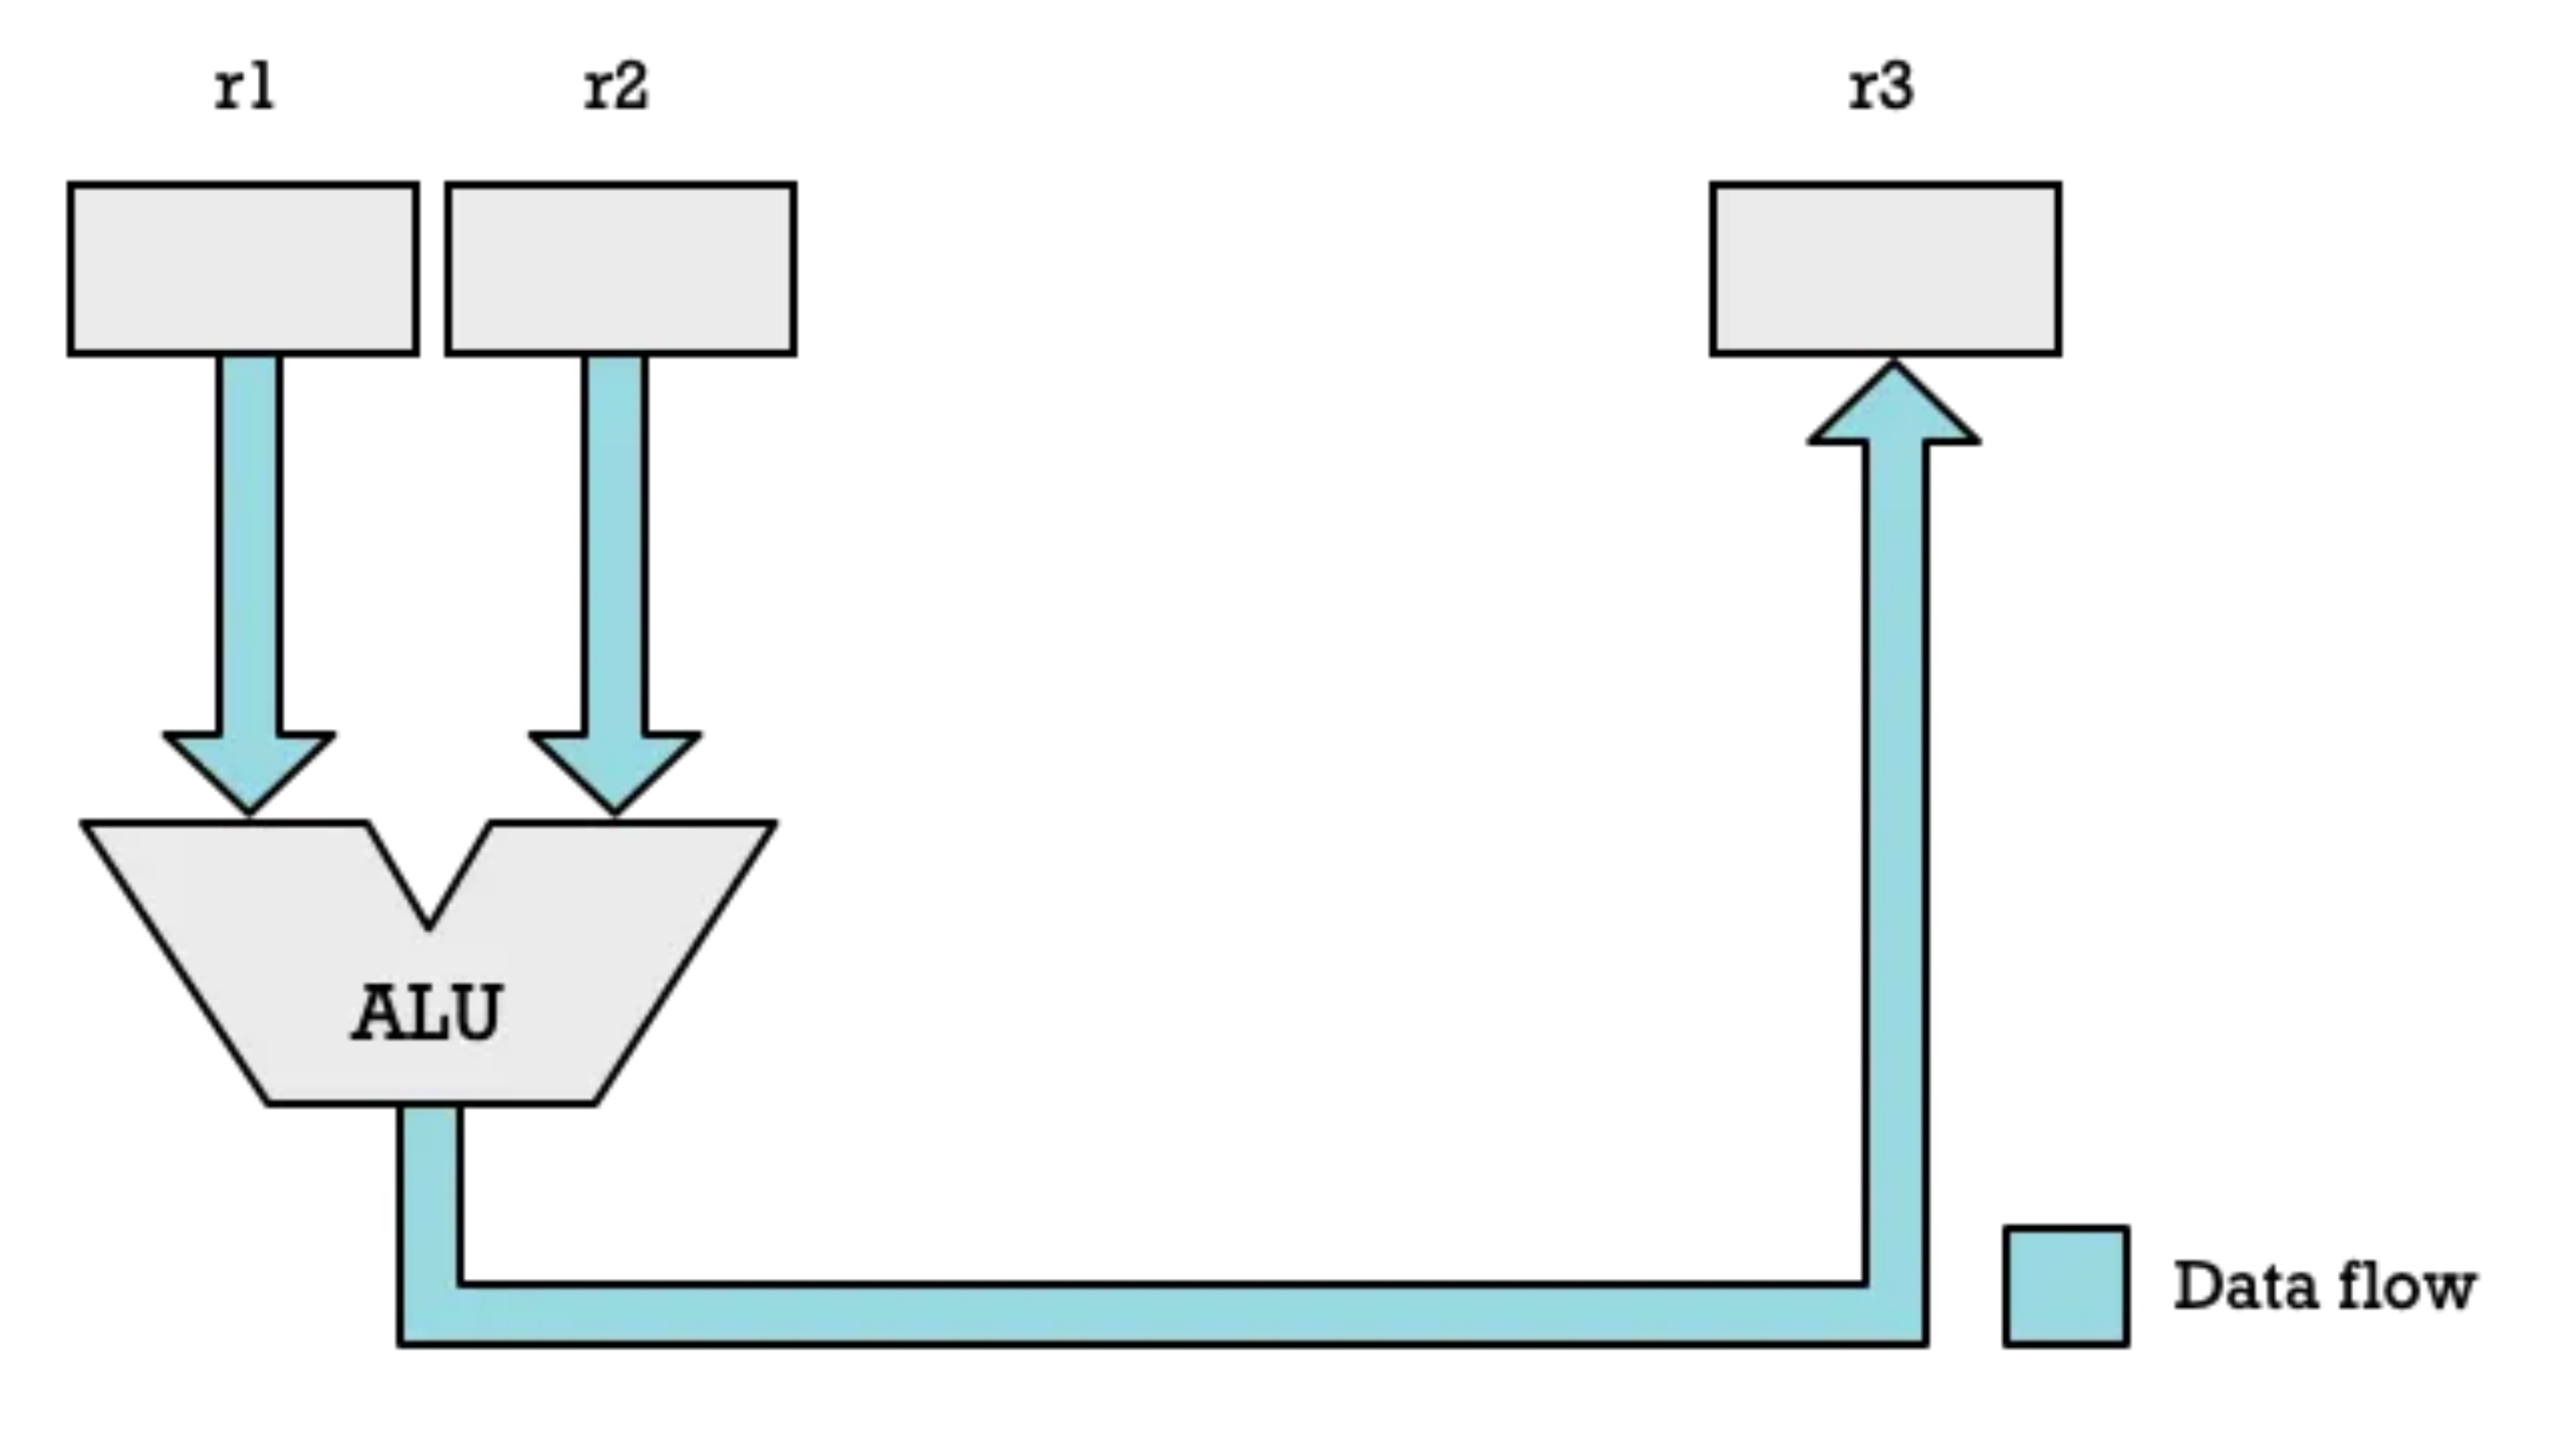
\includegraphics[scale=0.1]{ALU.png}
    \caption{Normally: Single Instruction, Single Data: https://itnext.io/vector-processing-on-cpus-and-gpus-compared-b1fab24343e6}
\end{figure}
When the CPU now executes the instructions like this, it reads two doubles into \texttt{r1} and \texttt{r2} respectively, multiplies them and writes them into \texttt{r3}. Then, it goes on to the next instruction and again loads two doubles and so on. In pseudo assembly code, this would look something like this:
\begin{figure}[H]
    \begin{subfigure}[t]{.5\textwidth}
        \texttt{Loop}:
        \begin{minted}[]{java}
result[i] = a[i] * b[i];
        \end{minted}
    \end{subfigure}%
    \begin{subfigure}[t]{.6\textwidth}
        \texttt{Corresponding Pseudo Assembly}:
        \begin{minted}[]{gas}
LOAD R1, (a) // load next double of 'a'
LOAD R2, (b) // load next double of 'b'
MUL R3, R1, R2 // R3 <- R1 * R2
        \end{minted}
    \end{subfigure}
\end{figure}
\noindent Now we want to enhance this CPU to enable SIMD instructions. For this, we need to increase the width of the registers and add another ALU. The registers \texttt{r1}, \texttt{r2} and \texttt{r3} we assumed so far are 64 bits wide (they hold exactly one double). Now, we assume we have registers \texttt{v1}, \texttt{v2} and \texttt{v3} that are 128 bits wide each. This means that we can put \textit{two} doubles into each such register. Now we can execute the following:
\begin{figure}[H]
    \centering
    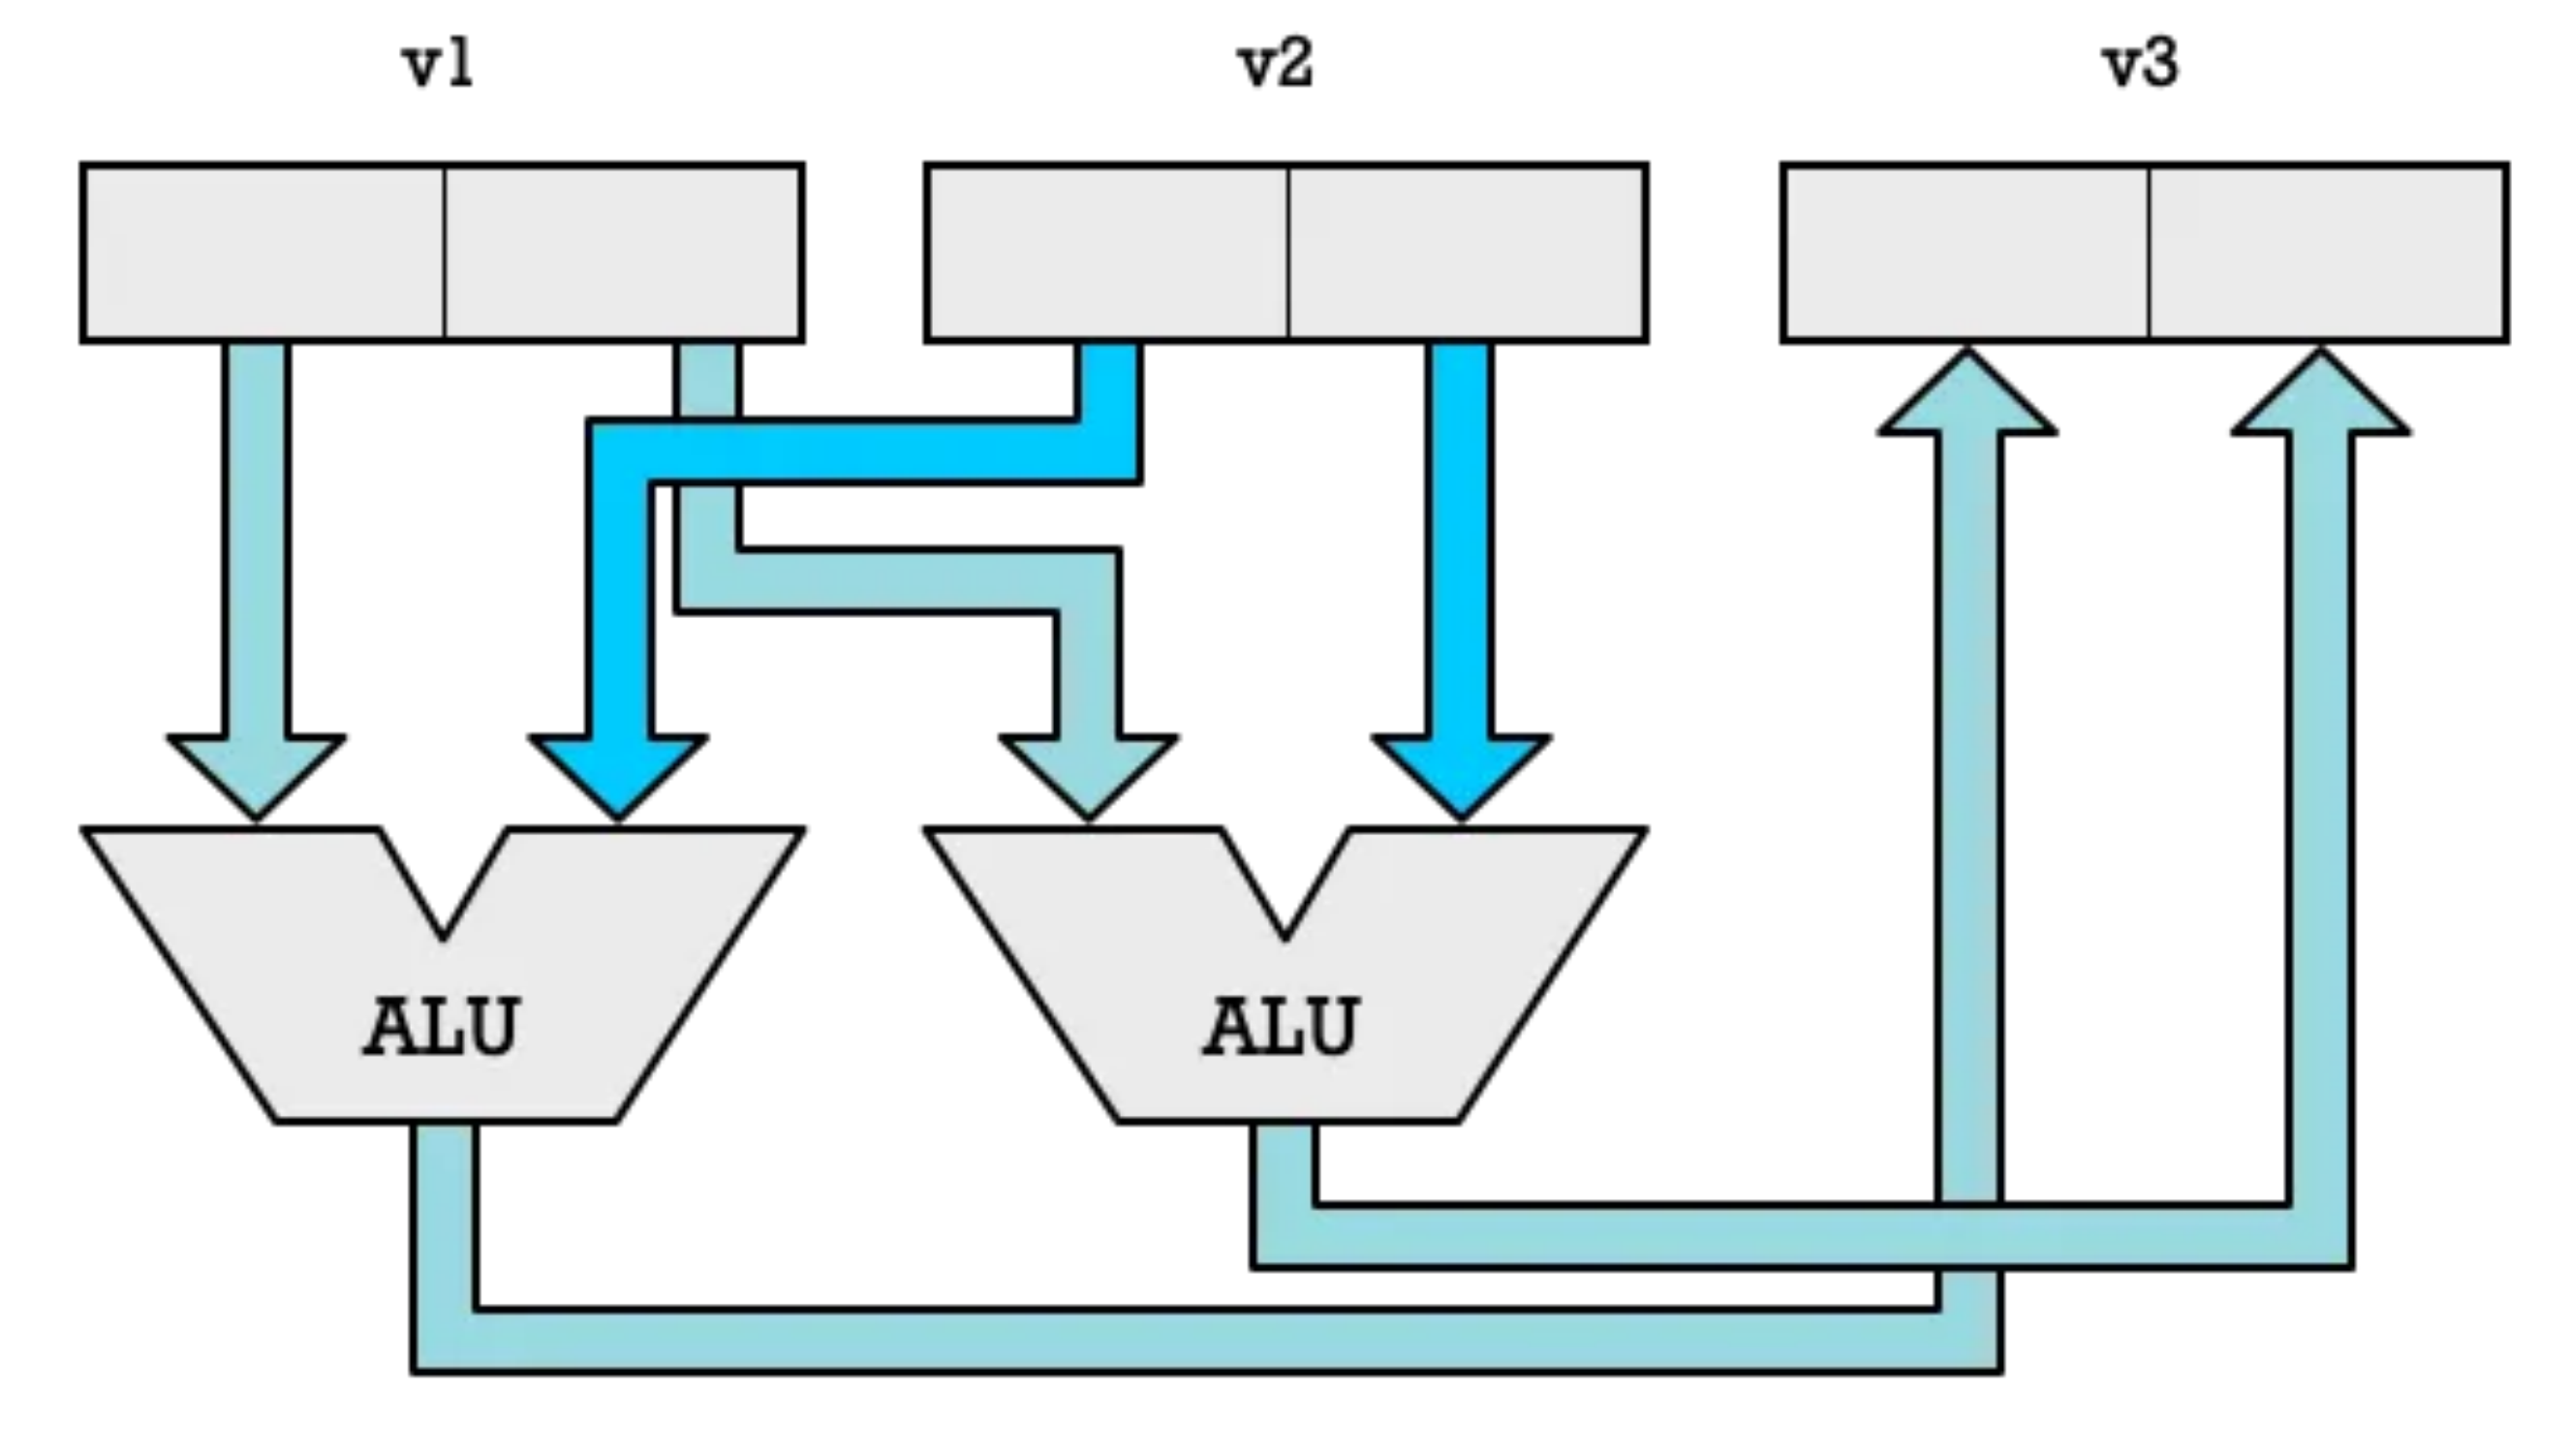
\includegraphics[scale=0.1]{SIMDalu.png}
    \caption{Single Instruction, Multiple Data: https://itnext.io/vector-processing-on-cpus-and-gpus-compared-b1fab24343e6}
\end{figure}
\noindent In one instruction, we can now load \textit{four} doubles, two into each of \texttt{v1} and \texttt{v2}. Then compute two multiplications in parallel using the two ALUs and write the two results into the register \texttt{v3}. In pseudo assembly code, this would then look something like this:
\begin{figure}[H]
    \begin{subfigure}[t]{.5\textwidth}
        \texttt{Unrolled Loop}:
        \begin{minted}[]{java}
result[i] = a[i] * b[i];
result[i+1] = a[i+1] * b[i+1];
        \end{minted}
    \end{subfigure}%
    \begin{subfigure}[t]{.6\textwidth}
        \texttt{Corresponding Pseudo Assembly}:
        \begin{minted}[]{gas}
VLOAD V1, (a) // load next two doubles of 'a'
VLOAD V2, (b) // load next two doubles of 'b'
VMUL V3, V1, V2 // V3 <- V1 * V2
        \end{minted}
    \end{subfigure}
\end{figure}
\noindent We introduced a special VMUL (vector multiply) instruction that uses special vector registers. We now know that these vector registers are just wider than normal registers and the vector instruction just uses multiple ALUs to compute the result in parallel.\\[3mm] This means that we can execute this loop approximately twice as fast using these twice as large registers, because we have only half the number of instructions.\\
But now think about what this means. SIMD happens on a single core. We can still create multiple threads and divide up the array to use even more parallelization. On one level, we can compute multiple parts of the array at the same time using multiple threads (that are hopefully scheduled on multiple cores at the same time). But on another level, in each core, multiple operations can be performed at the same time with SIMD. So, SIMD can be combined with multi-threading.

\subsubsection{How is Java Code Vectorized?}
So, if we have hardware that supports such special SIMD instructions, who actually optimizes the code to behave like this?\\
Let us quickly recap that in Java, the compiler translates our Java code to bytecode, which is agnostic of the underlying hardware. This means that such optimizations cannot happen at compile-time in Java, because the compiler cannot assume that the underlying hardware actually supports such instructions. But we also remember the JIT compiler that optimizes frequently executed code at \textit{runtime}. Vectorization is exactly such an optimization the JIT compiler can perform. Consider again the code from \ref{vectorization}. When we look at the machine code the JIT compiler generates at runtime (on an x86 system supporting SIMD instructions), we see the following:
\begin{minted}[]{gas}
vmovdqu   0x10(%r9, %rbx, 8), %ymm0
vmulpd    0x10(%rcx, %rbx, 8), %ymm0, %ymm0
vmovdqu   %ymm0, 0x10(%r13, %rbx, 8)
movslq    %ebx, %rsi
vmovdqu   0x30(%r9, %rsi, 8), %ymm0
vmulpd    0x30(%rcx, %rsi, 8), %ymm0, %ymm0
vmovdqu   %ymm0, 0x30(%r13, %rsi, 8)
vmovdqu   0x50(%r9, %rsi, 8), %ymm0
vmulpd    0x50(%rcx, %rsi, 8), %ymm0, %ymm0
vmovdqu   %ymm0, 0x50(%r13, %rsi, 8)
vmovdqu   0x70(%r9, %rsi, 8), %ymm0
vmulpd    0x70(%rcx, %rsi, 8), %ymm0, %ymm0
vmovdqu   %ymm0, 0x70(%r13, %rsi, 8)
\end{minted}
This is just a small part of the generated code, but we clearly see two things:
\begin{itemize}
  \item Vector instructions are used. The instructions starting with 'v' here are part of the AVX instruction set. AVX extends the x86 instruction set with vector (or SIMD) instructions for machines supporting it.
  \item We see that ymm registers are used. These are special registers that are 256-bits wide, meaning that they can hold \textit{four} doubles. This means (in conjunction with the vector instructions) four times less instructions compared to using normal 64-bit registers with normal (non-vector) instructions.
\end{itemize}
We can see that the JIT compiler successfully managed to optimize this loop at runtime to use the underlying hardware and vectorize it with SIMD without the programmer having to specify anything. So, we do not need to worry about exploiting this kind of parallelism as Java programmers. Note however that JIT only optimizes parts of the code that are executed a lot (for example a loop with many iterations). If the loop has only a few iterations in above code, the JIT compiler does not optimize it and hence the code does not use vector instructions even if the hardware supports it. Java provides special datastructures that give certain optimization guarantees, but we will not discuss these in this course.
\subsubsection{Concluding Vectorization}
What we remember about vectorization is the following:
\begin{itemize}
  \item Vectorization exploits ILP in the special case that the independent instructions are all of the same kind and operate on some vector-like datastructure (for example a for-loop performing an addition on each array element).
  \item Vectorization needs to be supported by the hardware. Usually in the form of larger registers and multiple execution units (in our example multiple ALUs). Then, there are special instructions that need to be used in order to make use of this.
  \item The compiler is responsible for translating these vectorizable code snippets into vector instructions for hardware with support for it. But in many languages vectorization is also exposed to the programmer via special libraries,  datastructures or the ability to hint to the compiler to use such vector instructions. In Java for example, there are special classes that provide guarantees about being mapped to vector instructions (if the underlying hardware supports it).
\end{itemize}
\subsection{Summary: ILP Approaches}
Let us now list a few different approaches towards exploiting ILP to get a feeling for how exactly they differ. This list is not exhaustive:
\begin{itemize}
  \item \textbf{Vectorization} exploits ILP in the special case where the independent instructions are all of the same kind on elements of a vector-like datastructure. The opportunity is found by the compiler, which combines multiple instructions (like an addition on multiple array elements) into a single vector instruction.
  \item \textbf{Pipelining} describes that the instruction execution is divided into multiple stages. The execution of independent instructions automatically happens in parallel (in the sense that they overlap in the pipeline). But to maximize the exploitation of ILP, the compiler and hardware need to ensure that dependent instructions have sufficient distance and these gaps get filled with independent instructions.
  \item \textbf{Superscalar execution} means that in each cycle, the CPU does not fetch just one, but \textit{multiple} instructions at once. This means that we need many additional execution units. We can imagine that in this approach, we have multiple mini-cores in one core, which can each fetch an instruction in every cycle and they each have their own execution path. To make use of all this hardware, the thread running on this core needs to have enough ILP, or else many of these mini-cores will have nothing to do. The difference to vectorization is that in superscalar execution, there are actually \textit{multiple} instructions that each have their own execution path on the core. Contrast that to vectorization, where the compiler just combines multiple instructions into a single one operating on larger operands.
\end{itemize}

\end{document}
